\documentclass[1p]{elsarticle_modified}
%\bibliographystyle{elsarticle-num}

%\usepackage[colorlinks]{hyperref}
%\usepackage{abbrmath_seonhwa} %\Abb, \Ascr, \Acal ,\Abf, \Afrak
\usepackage{amsfonts}
\usepackage{amssymb}
\usepackage{amsmath}
\usepackage{amsthm}
\usepackage{scalefnt}
\usepackage{amsbsy}
\usepackage{kotex}
\usepackage{caption}
\usepackage{subfig}
\usepackage{color}
\usepackage{graphicx}
\usepackage{xcolor} %% white, black, red, green, blue, cyan, magenta, yellow
\usepackage{float}
\usepackage{setspace}
\usepackage{hyperref}

\usepackage{tikz}
\usetikzlibrary{arrows}

\usepackage{multirow}
\usepackage{array} % fixed length table
\usepackage{hhline}

%%%%%%%%%%%%%%%%%%%%%
\makeatletter
\renewcommand*\env@matrix[1][\arraystretch]{%
	\edef\arraystretch{#1}%
	\hskip -\arraycolsep
	\let\@ifnextchar\new@ifnextchar
	\array{*\c@MaxMatrixCols c}}
\makeatother %https://tex.stackexchange.com/questions/14071/how-can-i-increase-the-line-spacing-in-a-matrix
%%%%%%%%%%%%%%%

\usepackage[normalem]{ulem}

\newcommand{\msout}[1]{\ifmmode\text{\sout{\ensuremath{#1}}}\else\sout{#1}\fi}
%SOURCE: \msout is \stkout macro in https://tex.stackexchange.com/questions/20609/strikeout-in-math-mode

\newcommand{\cancel}[1]{
	\ifmmode
	{\color{red}\msout{#1}}
	\else
	{\color{red}\sout{#1}}
	\fi
}

\newcommand{\add}[1]{
	{\color{blue}\uwave{#1}}
}

\newcommand{\replace}[2]{
	\ifmmode
	{\color{red}\msout{#1}}{\color{blue}\uwave{#2}}
	\else
	{\color{red}\sout{#1}}{\color{blue}\uwave{#2}}
	\fi
}

\newcommand{\Sol}{\mathcal{S}} %segment
\newcommand{\D}{D} %diagram
\newcommand{\A}{\mathcal{A}} %arc


%%%%%%%%%%%%%%%%%%%%%%%%%%%%%5 test

\def\sl{\operatorname{\textup{SL}}(2,\Cbb)}
\def\psl{\operatorname{\textup{PSL}}(2,\Cbb)}
\def\quan{\mkern 1mu \triangleright \mkern 1mu}

\theoremstyle{definition}
\newtheorem{thm}{Theorem}[section]
\newtheorem{prop}[thm]{Proposition}
\newtheorem{lem}[thm]{Lemma}
\newtheorem{ques}[thm]{Question}
\newtheorem{cor}[thm]{Corollary}
\newtheorem{defn}[thm]{Definition}
\newtheorem{exam}[thm]{Example}
\newtheorem{rmk}[thm]{Remark}
\newtheorem{alg}[thm]{Algorithm}

\newcommand{\I}{\sqrt{-1}}
\begin{document}

%\begin{frontmatter}
%
%\title{Boundary parabolic representations of knots up to 8 crossings}
%
%%% Group authors per affiliation:
%\author{Yunhi Cho} 
%\address{Department of Mathematics, University of Seoul, Seoul, Korea}
%\ead{yhcho@uos.ac.kr}
%
%
%\author{Seonhwa Kim} %\fnref{s_kim}}
%\address{Center for Geometry and Physics, Institute for Basic Science, Pohang, 37673, Korea}
%\ead{ryeona17@ibs.re.kr}
%
%\author{Hyuk Kim}
%\address{Department of Mathematical Sciences, Seoul National University, Seoul 08826, Korea}
%\ead{hyukkim@snu.ac.kr}
%
%\author{Seokbeom Yoon}
%\address{Department of Mathematical Sciences, Seoul National University, Seoul, 08826,  Korea}
%\ead{sbyoon15@snu.ac.kr}
%
%\begin{abstract}
%We find all boundary parabolic representation of knots up to 8 crossings.
%
%\end{abstract}
%\begin{keyword}
%    \MSC[2010] 57M25 
%\end{keyword}
%
%\end{frontmatter}

%\linenumbers
%\tableofcontents
%
\newcommand\colored[1]{\textcolor{white}{\rule[-0.35ex]{0.8em}{1.4ex}}\kern-0.8em\color{red} #1}%
%\newcommand\colored[1]{\textcolor{white}{ #1}\kern-2.17ex	\textcolor{white}{ #1}\kern-1.81ex	\textcolor{white}{ #1}\kern-2.15ex\color{red}#1	}

{\Large $\underline{11a_{104}~(K11a_{104})}$}

\setlength{\tabcolsep}{10pt}
\renewcommand{\arraystretch}{1.6}
\vspace{1cm}\begin{tabular}{m{100pt}>{\centering\arraybackslash}m{274pt}}
\multirow{5}{120pt}{
	\centering
	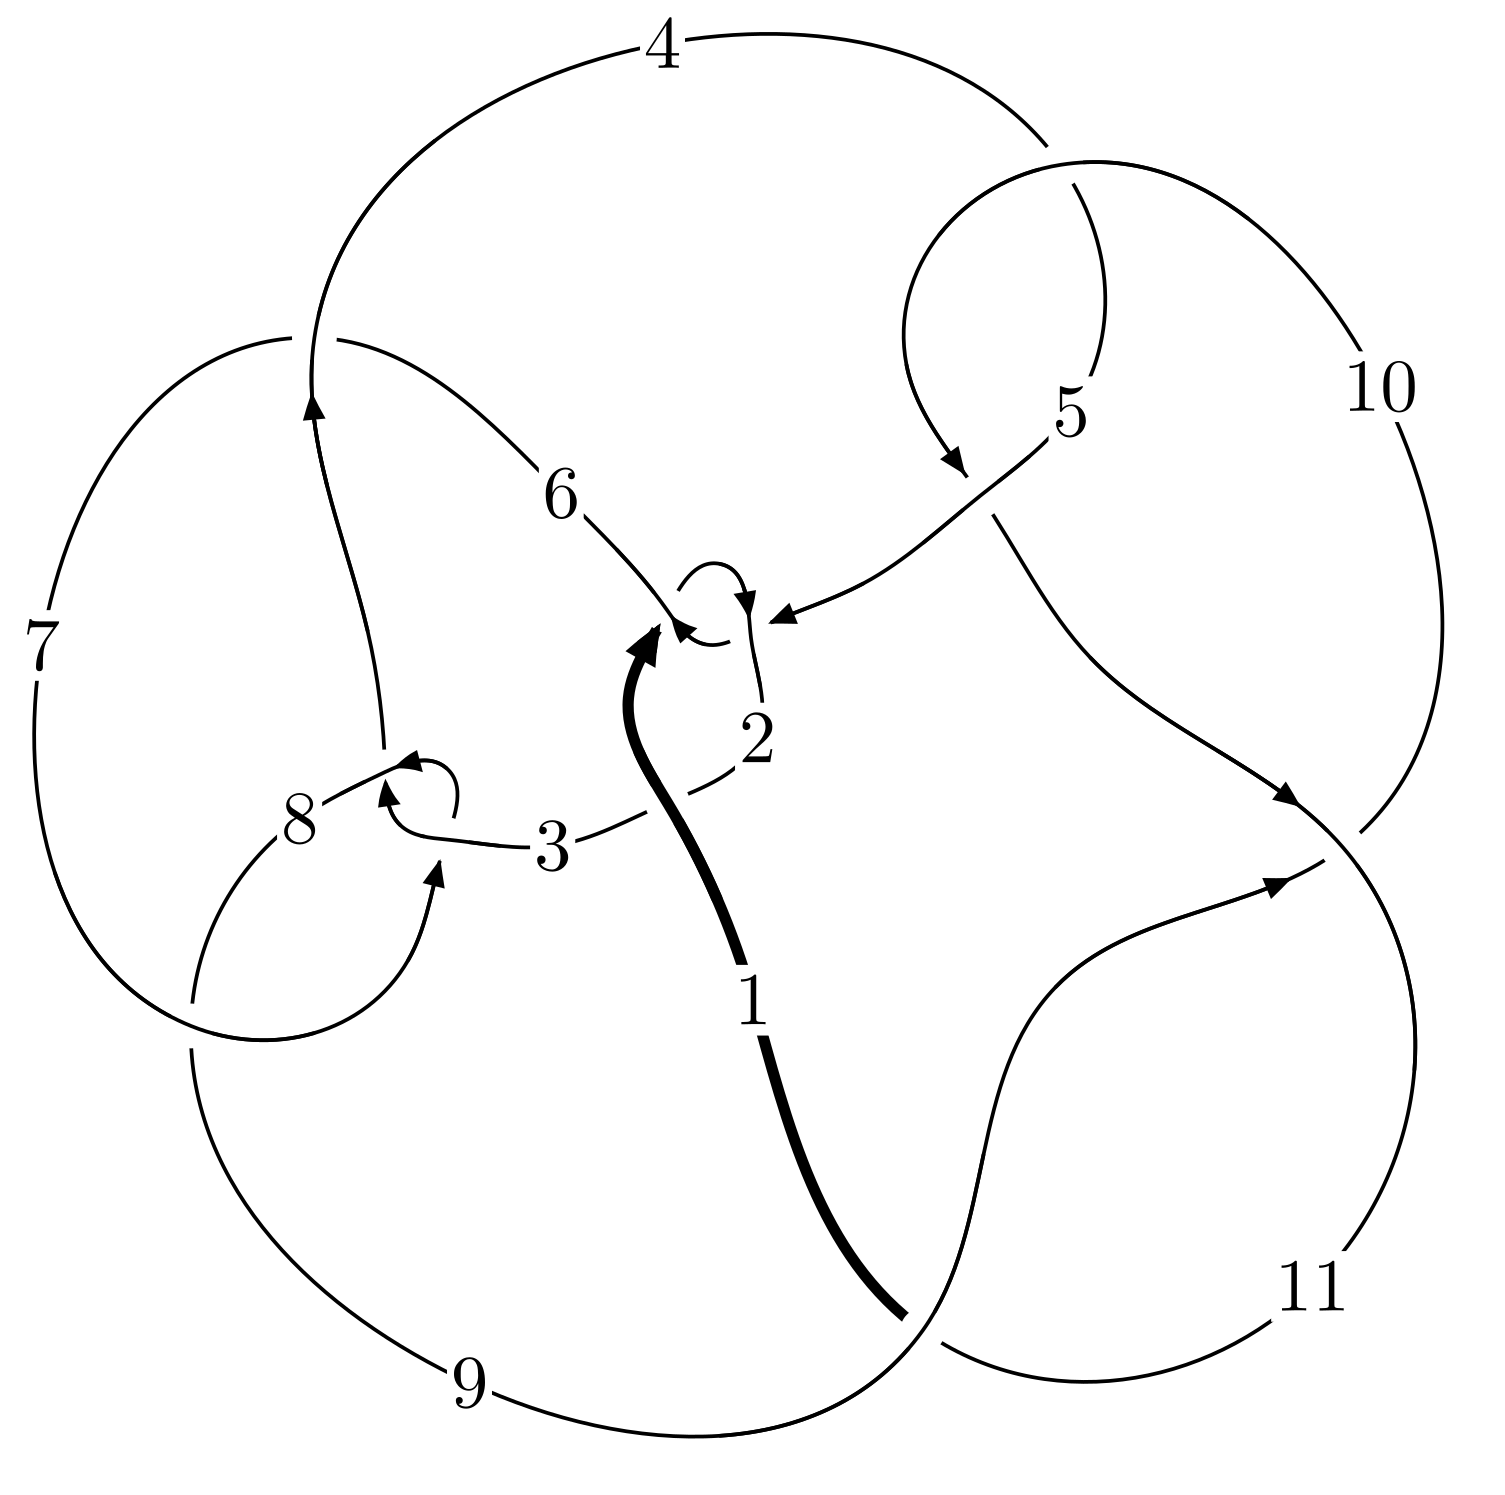
\includegraphics[width=112pt]{../../../GIT/diagram.site/Diagrams/png/353_11a_104.png}\\
\ \ \ A knot diagram\footnotemark}&
\allowdisplaybreaks
\textbf{Linearized knot diagam} \\
\cline{2-2}
 &
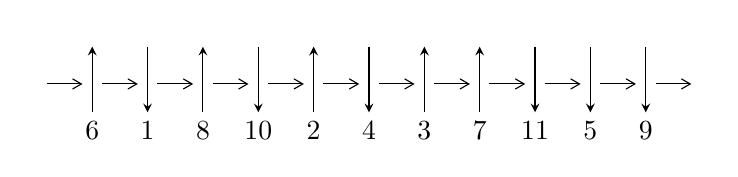
\begin{tikzpicture}[x=20pt, y=17pt]
	% nodes
	\node (C0) at (0, 0) {};
	\node (C1) at (1, 0) {};
	\node (C1U) at (1, +1) {};
	\node (C1D) at (1, -1) {6};

	\node (C2) at (2, 0) {};
	\node (C2U) at (2, +1) {};
	\node (C2D) at (2, -1) {1};

	\node (C3) at (3, 0) {};
	\node (C3U) at (3, +1) {};
	\node (C3D) at (3, -1) {8};

	\node (C4) at (4, 0) {};
	\node (C4U) at (4, +1) {};
	\node (C4D) at (4, -1) {10};

	\node (C5) at (5, 0) {};
	\node (C5U) at (5, +1) {};
	\node (C5D) at (5, -1) {2};

	\node (C6) at (6, 0) {};
	\node (C6U) at (6, +1) {};
	\node (C6D) at (6, -1) {4};

	\node (C7) at (7, 0) {};
	\node (C7U) at (7, +1) {};
	\node (C7D) at (7, -1) {3};

	\node (C8) at (8, 0) {};
	\node (C8U) at (8, +1) {};
	\node (C8D) at (8, -1) {7};

	\node (C9) at (9, 0) {};
	\node (C9U) at (9, +1) {};
	\node (C9D) at (9, -1) {11};

	\node (C10) at (10, 0) {};
	\node (C10U) at (10, +1) {};
	\node (C10D) at (10, -1) {5};

	\node (C11) at (11, 0) {};
	\node (C11U) at (11, +1) {};
	\node (C11D) at (11, -1) {9};
	\node (C12) at (12, 0) {};

	% arrows
	\draw[->,>={angle 60}]
	(C0) edge (C1) (C1) edge (C2) (C2) edge (C3) (C3) edge (C4) (C4) edge (C5) (C5) edge (C6) (C6) edge (C7) (C7) edge (C8) (C8) edge (C9) (C9) edge (C10) (C10) edge (C11) (C11) edge (C12) ;	\draw[->,>=stealth]
	(C1D) edge (C1U) (C2U) edge (C2D) (C3D) edge (C3U) (C4U) edge (C4D) (C5D) edge (C5U) (C6U) edge (C6D) (C7D) edge (C7U) (C8D) edge (C8U) (C9U) edge (C9D) (C10U) edge (C10D) (C11U) edge (C11D) ;
	\end{tikzpicture} \\
\hhline{~~} \\& 
\textbf{Solving Sequence} \\ \cline{2-2} 
 &
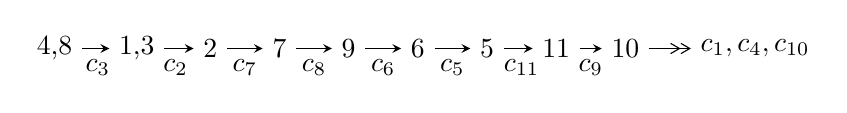
\begin{tikzpicture}[x=25pt, y=7pt]
	% node
	\node (A0) at (-1/8, 0) {4,8};
	\node (A1) at (17/16, 0) {1,3};
	\node (A2) at (17/8, 0) {2};
	\node (A3) at (25/8, 0) {7};
	\node (A4) at (33/8, 0) {9};
	\node (A5) at (41/8, 0) {6};
	\node (A6) at (49/8, 0) {5};
	\node (A7) at (57/8, 0) {11};
	\node (A8) at (65/8, 0) {10};
	\node (C1) at (1/2, -1) {$c_{3}$};
	\node (C2) at (13/8, -1) {$c_{2}$};
	\node (C3) at (21/8, -1) {$c_{7}$};
	\node (C4) at (29/8, -1) {$c_{8}$};
	\node (C5) at (37/8, -1) {$c_{6}$};
	\node (C6) at (45/8, -1) {$c_{5}$};
	\node (C7) at (53/8, -1) {$c_{11}$};
	\node (C8) at (61/8, -1) {$c_{9}$};
	\node (A9) at (10, 0) {$c_{1},c_{4},c_{10}$};

	% edge
	\draw[->,>=stealth]	
	(A0) edge (A1) (A1) edge (A2) (A2) edge (A3) (A3) edge (A4) (A4) edge (A5) (A5) edge (A6) (A6) edge (A7) (A7) edge (A8) ;
	\draw[->>,>={angle 60}]	
	(A8) edge (A9);
\end{tikzpicture} \\ 

\end{tabular} \\

\footnotetext{
The image of knot diagram is generated by the software ``\textbf{Draw programme}" developed by Andrew Bartholomew(\url{http://www.layer8.co.uk/maths/draw/index.htm\#Running-draw}), where we modified some parts for our purpose(\url{https://github.com/CATsTAILs/LinksPainter}).
}\phantom \\ \newline 
\centering \textbf{Ideals for irreducible components\footnotemark of $X_{\text{par}}$} 
 
\begin{align*}
I^u_{1}&=\langle 
-1.98593\times10^{23} u^{59}+4.69641\times10^{23} u^{58}+\cdots+1.04287\times10^{24} b+1.61518\times10^{24},\\
\phantom{I^u_{1}}&\phantom{= \langle  }3.87855\times10^{23} u^{59}-6.98208\times10^{22} u^{58}+\cdots+5.21436\times10^{23} a-1.87163\times10^{24},\;u^{60}+u^{59}+\cdots+2 u+1\rangle \\
I^u_{2}&=\langle 
b+u,\;- u^3+u^2+a+u-1,\;u^4- u^2+1\rangle \\
I^u_{3}&=\langle 
- u^7+u^5-2 u^3+b+u,\;- u^5+a- u,\;u^{10}-2 u^8+3 u^6- u^5-2 u^4+u^3+u^2- u+1\rangle \\
I^u_{4}&=\langle 
u^3+b- u,\;u^3+u^2+a-1,\;u^4- u^2+1\rangle \\
\\
\end{align*}
\raggedright * 4 irreducible components of $\dim_{\mathbb{C}}=0$, with total 78 representations.\\
\footnotetext{All coefficients of polynomials are rational numbers. But the coefficients are sometimes approximated in decimal forms when there is not enough margin.}
\newpage
\renewcommand{\arraystretch}{1}
\centering \section*{I. $I^u_{1}= \langle -1.99\times10^{23} u^{59}+4.70\times10^{23} u^{58}+\cdots+1.04\times10^{24} b+1.62\times10^{24},\;3.88\times10^{23} u^{59}-6.98\times10^{22} u^{58}+\cdots+5.21\times10^{23} a-1.87\times10^{24},\;u^{60}+u^{59}+\cdots+2 u+1 \rangle$}
\flushleft \textbf{(i) Arc colorings}\\
\begin{tabular}{m{7pt} m{180pt} m{7pt} m{180pt} }
\flushright $a_{4}=$&$\begin{pmatrix}1\\0\end{pmatrix}$ \\
\flushright $a_{8}=$&$\begin{pmatrix}0\\u\end{pmatrix}$ \\
\flushright $a_{1}=$&$\begin{pmatrix}-0.743821 u^{59}+0.133901 u^{58}+\cdots+0.842070 u+3.58938\\0.190429 u^{59}-0.450334 u^{58}+\cdots+0.891441 u-1.54878\end{pmatrix}$ \\
\flushright $a_{3}=$&$\begin{pmatrix}1\\u^2\end{pmatrix}$ \\
\flushright $a_{2}=$&$\begin{pmatrix}-1.04281 u^{59}-0.496774 u^{58}+\cdots+2.17071 u+3.63527\\1.12830 u^{59}+0.201741 u^{58}+\cdots+4.11950 u-0.780593\end{pmatrix}$ \\
\flushright $a_{7}=$&$\begin{pmatrix}- u\\- u^3+u\end{pmatrix}$ \\
\flushright $a_{9}=$&$\begin{pmatrix}u^3\\u^5- u^3+u\end{pmatrix}$ \\
\flushright $a_{6}=$&$\begin{pmatrix}- u^3\\- u^3+u\end{pmatrix}$ \\
\flushright $a_{5}=$&$\begin{pmatrix}-0.108079 u^{59}-1.37479 u^{58}+\cdots+6.24741 u-2.70886\\1.06440 u^{59}+0.333999 u^{58}+\cdots+3.85330 u-0.118756\end{pmatrix}$ \\
\flushright $a_{11}=$&$\begin{pmatrix}-1.14257 u^{59}-0.131348 u^{58}+\cdots+0.640675 u+3.85388\\1.04542 u^{59}+0.113508 u^{58}+\cdots+3.47215 u-0.882378\end{pmatrix}$ \\
\flushright $a_{10}=$&$\begin{pmatrix}0.423997 u^{59}-1.42113 u^{58}+\cdots+4.04661 u-5.47905\\0.233872 u^{59}-0.446189 u^{58}+\cdots+2.50575 u+0.581286\end{pmatrix}$\\ \flushright $a_{10}=$&$\begin{pmatrix}0.423997 u^{59}-1.42113 u^{58}+\cdots+4.04661 u-5.47905\\0.233872 u^{59}-0.446189 u^{58}+\cdots+2.50575 u+0.581286\end{pmatrix}$\\&\end{tabular}
\flushleft \textbf{(ii) Obstruction class $= -1$}\\~\\
\flushleft \textbf{(iii) Cusp Shapes $= \frac{1243755023537317604710317}{521436085097447226945316} u^{59}-\frac{113387074254912883763919}{260718042548723613472658} u^{58}+\cdots+\frac{5765858860985229173060379}{521436085097447226945316} u-\frac{629576893531561210869417}{130359021274361806736329}$}\\~\\
\newpage\renewcommand{\arraystretch}{1}
\flushleft \textbf{(iv) u-Polynomials at the component}\newline \\
\begin{tabular}{m{50pt}|m{274pt}}
Crossings & \hspace{64pt}u-Polynomials at each crossing \\
\hline $$\begin{aligned}c_{1},c_{5}\end{aligned}$$&$\begin{aligned}
&u^{60}+4 u^{59}+\cdots+20 u+4
\end{aligned}$\\
\hline $$\begin{aligned}c_{2}\end{aligned}$$&$\begin{aligned}
&u^{60}+28 u^{59}+\cdots+136 u+16
\end{aligned}$\\
\hline $$\begin{aligned}c_{3},c_{7}\end{aligned}$$&$\begin{aligned}
&u^{60}- u^{59}+\cdots-2 u+1
\end{aligned}$\\
\hline $$\begin{aligned}c_{4},c_{10}\end{aligned}$$&$\begin{aligned}
&u^{60}- u^{59}+\cdots+8 u+1
\end{aligned}$\\
\hline $$\begin{aligned}c_{6}\end{aligned}$$&$\begin{aligned}
&u^{60}-3 u^{59}+\cdots-628 u+261
\end{aligned}$\\
\hline $$\begin{aligned}c_{8}\end{aligned}$$&$\begin{aligned}
&u^{60}-31 u^{59}+\cdots-6 u+1
\end{aligned}$\\
\hline $$\begin{aligned}c_{9},c_{11}\end{aligned}$$&$\begin{aligned}
&u^{60}+19 u^{59}+\cdots+54 u+1
\end{aligned}$\\
\hline
\end{tabular}\\~\\
\newpage\renewcommand{\arraystretch}{1}
\flushleft \textbf{(v) Riley Polynomials at the component}\newline \\
\begin{tabular}{m{50pt}|m{274pt}}
Crossings & \hspace{64pt}Riley Polynomials at each crossing \\
\hline $$\begin{aligned}c_{1},c_{5}\end{aligned}$$&$\begin{aligned}
&y^{60}+28 y^{59}+\cdots+136 y+16
\end{aligned}$\\
\hline $$\begin{aligned}c_{2}\end{aligned}$$&$\begin{aligned}
&y^{60}+12 y^{59}+\cdots+13024 y+256
\end{aligned}$\\
\hline $$\begin{aligned}c_{3},c_{7}\end{aligned}$$&$\begin{aligned}
&y^{60}-31 y^{59}+\cdots-6 y+1
\end{aligned}$\\
\hline $$\begin{aligned}c_{4},c_{10}\end{aligned}$$&$\begin{aligned}
&y^{60}-19 y^{59}+\cdots-54 y+1
\end{aligned}$\\
\hline $$\begin{aligned}c_{6}\end{aligned}$$&$\begin{aligned}
&y^{60}+29 y^{59}+\cdots-446062 y+68121
\end{aligned}$\\
\hline $$\begin{aligned}c_{8}\end{aligned}$$&$\begin{aligned}
&y^{60}+y^{59}+\cdots+38 y+1
\end{aligned}$\\
\hline $$\begin{aligned}c_{9},c_{11}\end{aligned}$$&$\begin{aligned}
&y^{60}+49 y^{59}+\cdots-562 y+1
\end{aligned}$\\
\hline
\end{tabular}\\~\\
\newpage\flushleft \textbf{(vi) Complex Volumes and Cusp Shapes}
$$\begin{array}{c|c|c}  
\text{Solutions to }I^u_{1}& \I (\text{vol} + \sqrt{-1}CS) & \text{Cusp shape}\\
 \hline 
\begin{aligned}
u &= \phantom{-}0.903831 + 0.403972 I \\
a &= \phantom{-}1.269250 - 0.398175 I \\
b &= \phantom{-}1.057390 + 0.767924 I\end{aligned}
 & \phantom{-}0.07179 + 4.23224 I & \phantom{-}2.32754 - 7.48197 I \\ \hline\begin{aligned}
u &= \phantom{-}0.903831 - 0.403972 I \\
a &= \phantom{-}1.269250 + 0.398175 I \\
b &= \phantom{-}1.057390 - 0.767924 I\end{aligned}
 & \phantom{-}0.07179 - 4.23224 I & \phantom{-}2.32754 + 7.48197 I \\ \hline\begin{aligned}
u &= -0.711823 + 0.747660 I \\
a &= -0.406775 - 0.002759 I \\
b &= -0.634669 - 0.607886 I\end{aligned}
 & -0.59950 - 7.44517 I & -1.81786 + 8.61499 I \\ \hline\begin{aligned}
u &= -0.711823 - 0.747660 I \\
a &= -0.406775 + 0.002759 I \\
b &= -0.634669 + 0.607886 I\end{aligned}
 & -0.59950 + 7.44517 I & -1.81786 - 8.61499 I \\ \hline\begin{aligned}
u &= \phantom{-}0.804581 + 0.489615 I \\
a &= \phantom{-}0.265943 - 0.865672 I \\
b &= -0.177298 + 0.044040 I\end{aligned}
 & -1.74326 + 2.05593 I & -4.38675 - 3.92763 I \\ \hline\begin{aligned}
u &= \phantom{-}0.804581 - 0.489615 I \\
a &= \phantom{-}0.265943 + 0.865672 I \\
b &= -0.177298 - 0.044040 I\end{aligned}
 & -1.74326 - 2.05593 I & -4.38675 + 3.92763 I \\ \hline\begin{aligned}
u &= \phantom{-}0.859520 + 0.676363 I \\
a &= \phantom{-}0.964914 - 0.424298 I \\
b &= \phantom{-}0.480610 + 0.345118 I\end{aligned}
 & \phantom{-}0.30698 + 3.25660 I & \phantom{-0.000000 } 0. - 2.79575 I \\ \hline\begin{aligned}
u &= \phantom{-}0.859520 - 0.676363 I \\
a &= \phantom{-}0.964914 + 0.424298 I \\
b &= \phantom{-}0.480610 - 0.345118 I\end{aligned}
 & \phantom{-}0.30698 - 3.25660 I & \phantom{-0.000000 -}0. + 2.79575 I \\ \hline\begin{aligned}
u &= -0.311259 + 0.850032 I \\
a &= -0.321328 - 0.147611 I \\
b &= -0.73288 + 1.72138 I\end{aligned}
 & \phantom{-}1.72838 + 10.40930 I & -1.97334 - 6.85461 I \\ \hline\begin{aligned}
u &= -0.311259 - 0.850032 I \\
a &= -0.321328 + 0.147611 I \\
b &= -0.73288 - 1.72138 I\end{aligned}
 & \phantom{-}1.72838 - 10.40930 I & -1.97334 + 6.85461 I\\
 \hline 
 \end{array}$$\newpage$$\begin{array}{c|c|c}  
\text{Solutions to }I^u_{1}& \I (\text{vol} + \sqrt{-1}CS) & \text{Cusp shape}\\
 \hline 
\begin{aligned}
u &= -0.865604 + 0.182246 I \\
a &= \phantom{-}0.606319 + 0.298940 I \\
b &= \phantom{-}0.748686 - 0.118582 I\end{aligned}
 & \phantom{-}1.47274 - 0.43868 I & \phantom{-}6.40126 + 0.73626 I \\ \hline\begin{aligned}
u &= -0.865604 - 0.182246 I \\
a &= \phantom{-}0.606319 - 0.298940 I \\
b &= \phantom{-}0.748686 + 0.118582 I\end{aligned}
 & \phantom{-}1.47274 + 0.43868 I & \phantom{-}6.40126 - 0.73626 I \\ \hline\begin{aligned}
u &= \phantom{-}0.272152 + 0.836204 I \\
a &= -0.196628 + 0.183823 I \\
b &= -0.68548 - 1.62535 I\end{aligned}
 & \phantom{-}2.73192 - 4.52059 I & -0.21234 + 2.21964 I \\ \hline\begin{aligned}
u &= \phantom{-}0.272152 - 0.836204 I \\
a &= -0.196628 - 0.183823 I \\
b &= -0.68548 + 1.62535 I\end{aligned}
 & \phantom{-}2.73192 + 4.52059 I & -0.21234 - 2.21964 I \\ \hline\begin{aligned}
u &= -0.568756 + 0.644224 I \\
a &= -0.676994 + 0.457932 I \\
b &= -0.717357 - 0.302413 I\end{aligned}
 & -5.04608 - 2.62544 I & -9.38058 + 3.85437 I \\ \hline\begin{aligned}
u &= -0.568756 - 0.644224 I \\
a &= -0.676994 - 0.457932 I \\
b &= -0.717357 + 0.302413 I\end{aligned}
 & -5.04608 + 2.62544 I & -9.38058 - 3.85437 I \\ \hline\begin{aligned}
u &= -0.993886 + 0.578329 I \\
a &= \phantom{-}0.955168 + 0.848146 I \\
b &= \phantom{-}0.415861 + 0.077795 I\end{aligned}
 & -3.79990 - 2.15619 I & \phantom{-0.000000 } 0 \\ \hline\begin{aligned}
u &= -0.993886 - 0.578329 I \\
a &= \phantom{-}0.955168 - 0.848146 I \\
b &= \phantom{-}0.415861 - 0.077795 I\end{aligned}
 & -3.79990 + 2.15619 I & \phantom{-0.000000 } 0 \\ \hline\begin{aligned}
u &= \phantom{-}1.054100 + 0.478696 I \\
a &= \phantom{-}1.15838 + 1.04975 I \\
b &= \phantom{-}0.14104 + 1.62136 I\end{aligned}
 & \phantom{-}0.06948 + 4.64990 I & \phantom{-0.000000 } 0 \\ \hline\begin{aligned}
u &= \phantom{-}1.054100 - 0.478696 I \\
a &= \phantom{-}1.15838 - 1.04975 I \\
b &= \phantom{-}0.14104 - 1.62136 I\end{aligned}
 & \phantom{-}0.06948 - 4.64990 I & \phantom{-0.000000 } 0\\
 \hline 
 \end{array}$$\newpage$$\begin{array}{c|c|c}  
\text{Solutions to }I^u_{1}& \I (\text{vol} + \sqrt{-1}CS) & \text{Cusp shape}\\
 \hline 
\begin{aligned}
u &= \phantom{-}1.080780 + 0.429889 I \\
a &= \phantom{-}0.96586 - 1.23049 I \\
b &= \phantom{-}0.319260 - 0.470303 I\end{aligned}
 & \phantom{-}0.799952 + 0.856311 I & \phantom{-0.000000 } 0 \\ \hline\begin{aligned}
u &= \phantom{-}1.080780 - 0.429889 I \\
a &= \phantom{-}0.96586 + 1.23049 I \\
b &= \phantom{-}0.319260 + 0.470303 I\end{aligned}
 & \phantom{-}0.799952 - 0.856311 I & \phantom{-0.000000 } 0 \\ \hline\begin{aligned}
u &= \phantom{-}0.210101 + 0.809324 I \\
a &= \phantom{-}0.740667 - 0.015178 I \\
b &= \phantom{-}0.105661 + 1.028970 I\end{aligned}
 & \phantom{-}3.79462 - 4.80277 I & \phantom{-}0.86247 + 2.90071 I \\ \hline\begin{aligned}
u &= \phantom{-}0.210101 - 0.809324 I \\
a &= \phantom{-}0.740667 + 0.015178 I \\
b &= \phantom{-}0.105661 - 1.028970 I\end{aligned}
 & \phantom{-}3.79462 + 4.80277 I & \phantom{-}0.86247 - 2.90071 I \\ \hline\begin{aligned}
u &= -1.116060 + 0.386772 I \\
a &= \phantom{-}1.21794 - 1.49474 I \\
b &= \phantom{-}0.00600 - 1.76185 I\end{aligned}
 & \phantom{-}3.40701 - 1.33155 I & \phantom{-0.000000 } 0 \\ \hline\begin{aligned}
u &= -1.116060 - 0.386772 I \\
a &= \phantom{-}1.21794 + 1.49474 I \\
b &= \phantom{-}0.00600 + 1.76185 I\end{aligned}
 & \phantom{-}3.40701 + 1.33155 I & \phantom{-0.000000 } 0 \\ \hline\begin{aligned}
u &= -0.144728 + 0.798733 I \\
a &= \phantom{-}0.670793 + 0.046459 I \\
b &= \phantom{-}0.000564 - 1.065940 I\end{aligned}
 & \phantom{-}4.37725 - 1.04056 I & \phantom{-}1.90122 + 2.49141 I \\ \hline\begin{aligned}
u &= -0.144728 - 0.798733 I \\
a &= \phantom{-}0.670793 - 0.046459 I \\
b &= \phantom{-}0.000564 + 1.065940 I\end{aligned}
 & \phantom{-}4.37725 + 1.04056 I & \phantom{-}1.90122 - 2.49141 I \\ \hline\begin{aligned}
u &= -1.094520 + 0.479352 I \\
a &= \phantom{-}1.03063 + 1.15150 I \\
b &= \phantom{-}0.414981 + 0.408719 I\end{aligned}
 & \phantom{-}0.42302 - 6.32152 I & \phantom{-0.000000 } 0 \\ \hline\begin{aligned}
u &= -1.094520 - 0.479352 I \\
a &= \phantom{-}1.03063 - 1.15150 I \\
b &= \phantom{-}0.414981 - 0.408719 I\end{aligned}
 & \phantom{-}0.42302 + 6.32152 I & \phantom{-0.000000 } 0\\
 \hline 
 \end{array}$$\newpage$$\begin{array}{c|c|c}  
\text{Solutions to }I^u_{1}& \I (\text{vol} + \sqrt{-1}CS) & \text{Cusp shape}\\
 \hline 
\begin{aligned}
u &= -0.339818 + 0.708730 I \\
a &= -0.355808 - 0.663857 I \\
b &= -1.06664 + 1.47014 I\end{aligned}
 & -4.04431 + 4.50698 I & -7.28201 - 4.72365 I \\ \hline\begin{aligned}
u &= -0.339818 - 0.708730 I \\
a &= -0.355808 + 0.663857 I \\
b &= -1.06664 - 1.47014 I\end{aligned}
 & -4.04431 - 4.50698 I & -7.28201 + 4.72365 I \\ \hline\begin{aligned}
u &= \phantom{-}1.128850 + 0.492143 I \\
a &= -0.52081 - 2.12283 I \\
b &= \phantom{-}1.32820 - 1.57388 I\end{aligned}
 & \phantom{-}2.66218 + 6.38495 I & \phantom{-0.000000 } 0 \\ \hline\begin{aligned}
u &= \phantom{-}1.128850 - 0.492143 I \\
a &= -0.52081 + 2.12283 I \\
b &= \phantom{-}1.32820 + 1.57388 I\end{aligned}
 & \phantom{-}2.66218 - 6.38495 I & \phantom{-0.000000 } 0 \\ \hline\begin{aligned}
u &= \phantom{-}1.216210 + 0.225171 I \\
a &= \phantom{-}1.10465 + 1.80874 I \\
b &= -0.02516 + 1.64383 I\end{aligned}
 & \phantom{-}6.74362 - 7.16149 I & \phantom{-0.000000 } 0 \\ \hline\begin{aligned}
u &= \phantom{-}1.216210 - 0.225171 I \\
a &= \phantom{-}1.10465 - 1.80874 I \\
b &= -0.02516 - 1.64383 I\end{aligned}
 & \phantom{-}6.74362 + 7.16149 I & \phantom{-0.000000 } 0 \\ \hline\begin{aligned}
u &= -1.112300 + 0.548551 I \\
a &= -0.84176 + 2.42145 I \\
b &= \phantom{-}1.34785 + 2.08020 I\end{aligned}
 & -1.78746 - 9.32372 I & \phantom{-0.000000 } 0 \\ \hline\begin{aligned}
u &= -1.112300 - 0.548551 I \\
a &= -0.84176 - 2.42145 I \\
b &= \phantom{-}1.34785 - 2.08020 I\end{aligned}
 & -1.78746 + 9.32372 I & \phantom{-0.000000 } 0 \\ \hline\begin{aligned}
u &= -1.212780 + 0.262306 I \\
a &= \phantom{-}1.10372 - 1.77604 I \\
b &= -0.02790 - 1.67922 I\end{aligned}
 & \phantom{-}7.49647 + 1.10876 I & \phantom{-0.000000 } 0 \\ \hline\begin{aligned}
u &= -1.212780 - 0.262306 I \\
a &= \phantom{-}1.10372 + 1.77604 I \\
b &= -0.02790 + 1.67922 I\end{aligned}
 & \phantom{-}7.49647 - 1.10876 I & \phantom{-0.000000 } 0\\
 \hline 
 \end{array}$$\newpage$$\begin{array}{c|c|c}  
\text{Solutions to }I^u_{1}& \I (\text{vol} + \sqrt{-1}CS) & \text{Cusp shape}\\
 \hline 
\begin{aligned}
u &= -1.207080 + 0.312500 I \\
a &= -0.432975 + 1.070400 I \\
b &= \phantom{-}0.694965 + 0.705252 I\end{aligned}
 & \phantom{-}8.19036 + 1.16781 I & \phantom{-0.000000 } 0 \\ \hline\begin{aligned}
u &= -1.207080 - 0.312500 I \\
a &= -0.432975 - 1.070400 I \\
b &= \phantom{-}0.694965 - 0.705252 I\end{aligned}
 & \phantom{-}8.19036 - 1.16781 I & \phantom{-0.000000 } 0 \\ \hline\begin{aligned}
u &= \phantom{-}1.207510 + 0.352417 I \\
a &= -0.476722 - 1.234610 I \\
b &= \phantom{-}0.746612 - 0.850988 I\end{aligned}
 & \phantom{-}8.50343 + 4.91869 I & \phantom{-0.000000 } 0 \\ \hline\begin{aligned}
u &= \phantom{-}1.207510 - 0.352417 I \\
a &= -0.476722 + 1.234610 I \\
b &= \phantom{-}0.746612 + 0.850988 I\end{aligned}
 & \phantom{-}8.50343 - 4.91869 I & \phantom{-0.000000 } 0 \\ \hline\begin{aligned}
u &= -1.179680 + 0.510060 I \\
a &= \phantom{-}0.83860 - 1.38186 I \\
b &= -0.05723 - 1.67219 I\end{aligned}
 & \phantom{-}7.41896 - 3.74798 I & \phantom{-0.000000 } 0 \\ \hline\begin{aligned}
u &= -1.179680 - 0.510060 I \\
a &= \phantom{-}0.83860 + 1.38186 I \\
b &= -0.05723 + 1.67219 I\end{aligned}
 & \phantom{-}7.41896 + 3.74798 I & \phantom{-0.000000 } 0 \\ \hline\begin{aligned}
u &= \phantom{-}1.173440 + 0.538194 I \\
a &= \phantom{-}0.77481 + 1.33580 I \\
b &= -0.07894 + 1.64826 I\end{aligned}
 & \phantom{-}6.63935 + 9.77588 I & \phantom{-0.000000 } 0 \\ \hline\begin{aligned}
u &= \phantom{-}1.173440 - 0.538194 I \\
a &= \phantom{-}0.77481 - 1.33580 I \\
b &= -0.07894 - 1.64826 I\end{aligned}
 & \phantom{-}6.63935 - 9.77588 I & \phantom{-0.000000 } 0 \\ \hline\begin{aligned}
u &= \phantom{-}1.169570 + 0.567517 I \\
a &= -1.03891 - 2.10766 I \\
b &= \phantom{-}0.89396 - 2.01477 I\end{aligned}
 & \phantom{-}5.40914 + 9.70793 I & \phantom{-0.000000 } 0 \\ \hline\begin{aligned}
u &= \phantom{-}1.169570 - 0.567517 I \\
a &= -1.03891 + 2.10766 I \\
b &= \phantom{-}0.89396 + 2.01477 I\end{aligned}
 & \phantom{-}5.40914 - 9.70793 I & \phantom{-0.000000 } 0\\
 \hline 
 \end{array}$$\newpage$$\begin{array}{c|c|c}  
\text{Solutions to }I^u_{1}& \I (\text{vol} + \sqrt{-1}CS) & \text{Cusp shape}\\
 \hline 
\begin{aligned}
u &= -1.163930 + 0.586363 I \\
a &= -1.12390 + 2.15224 I \\
b &= \phantom{-}0.86334 + 2.13698 I\end{aligned}
 & \phantom{-}4.2834 - 15.7183 I & \phantom{-0.000000 } 0 \\ \hline\begin{aligned}
u &= -1.163930 - 0.586363 I \\
a &= -1.12390 - 2.15224 I \\
b &= \phantom{-}0.86334 - 2.13698 I\end{aligned}
 & \phantom{-}4.2834 + 15.7183 I & \phantom{-0.000000 } 0 \\ \hline\begin{aligned}
u &= \phantom{-}0.429148 + 0.530188 I \\
a &= \phantom{-}0.903246 - 0.132373 I \\
b &= \phantom{-}0.249666 + 0.565526 I\end{aligned}
 & -1.72663 - 0.52634 I & -4.33031 + 0.44248 I \\ \hline\begin{aligned}
u &= \phantom{-}0.429148 - 0.530188 I \\
a &= \phantom{-}0.903246 + 0.132373 I \\
b &= \phantom{-}0.249666 - 0.565526 I\end{aligned}
 & -1.72663 + 0.52634 I & -4.33031 - 0.44248 I \\ \hline\begin{aligned}
u &= \phantom{-}0.637665 + 0.183912 I \\
a &= -0.11399 - 1.94899 I \\
b &= -0.738126 - 0.352707 I\end{aligned}
 & -1.24161 + 2.23775 I & -0.61490 - 2.94515 I \\ \hline\begin{aligned}
u &= \phantom{-}0.637665 - 0.183912 I \\
a &= -0.11399 + 1.94899 I \\
b &= -0.738126 + 0.352707 I\end{aligned}
 & -1.24161 - 2.23775 I & -0.61490 + 2.94515 I \\ \hline\begin{aligned}
u &= -0.362759 + 0.416974 I \\
a &= \phantom{-}0.17781 - 1.91746 I \\
b &= -1.45310 + 0.56258 I\end{aligned}
 & -2.02553 - 1.88873 I & -4.74604 + 1.07620 I \\ \hline\begin{aligned}
u &= -0.362759 - 0.416974 I \\
a &= \phantom{-}0.17781 + 1.91746 I \\
b &= -1.45310 - 0.56258 I\end{aligned}
 & -2.02553 + 1.88873 I & -4.74604 - 1.07620 I \\ \hline\begin{aligned}
u &= -0.262460 + 0.449731 I \\
a &= -1.74210 + 0.98505 I \\
b &= -0.919872 - 0.033488 I\end{aligned}
 & -1.87789 + 2.29756 I & -4.03068 - 3.27403 I \\ \hline\begin{aligned}
u &= -0.262460 - 0.449731 I \\
a &= -1.74210 - 0.98505 I \\
b &= -0.919872 + 0.033488 I\end{aligned}
 & -1.87789 - 2.29756 I & -4.03068 + 3.27403 I\\
 \hline 
 \end{array}$$\newpage\newpage\renewcommand{\arraystretch}{1}
\centering \section*{II. $I^u_{2}= \langle b+u,\;- u^3+u^2+a+u-1,\;u^4- u^2+1 \rangle$}
\flushleft \textbf{(i) Arc colorings}\\
\begin{tabular}{m{7pt} m{180pt} m{7pt} m{180pt} }
\flushright $a_{4}=$&$\begin{pmatrix}1\\0\end{pmatrix}$ \\
\flushright $a_{8}=$&$\begin{pmatrix}0\\u\end{pmatrix}$ \\
\flushright $a_{1}=$&$\begin{pmatrix}u^3- u^2- u+1\\- u\end{pmatrix}$ \\
\flushright $a_{3}=$&$\begin{pmatrix}1\\u^2\end{pmatrix}$ \\
\flushright $a_{2}=$&$\begin{pmatrix}u^3- u^2- u+2\\u^2- u\end{pmatrix}$ \\
\flushright $a_{7}=$&$\begin{pmatrix}- u\\- u^3+u\end{pmatrix}$ \\
\flushright $a_{9}=$&$\begin{pmatrix}u^3\\0\end{pmatrix}$ \\
\flushright $a_{6}=$&$\begin{pmatrix}- u^3\\- u^3+u\end{pmatrix}$ \\
\flushright $a_{5}=$&$\begin{pmatrix}- u^2+u\\- u^2+1\end{pmatrix}$ \\
\flushright $a_{11}=$&$\begin{pmatrix}u^3- u^2+1\\- u\end{pmatrix}$ \\
\flushright $a_{10}=$&$\begin{pmatrix}u^3- u^2+u\\u^3- u\end{pmatrix}$\\ \flushright $a_{10}=$&$\begin{pmatrix}u^3- u^2+u\\u^3- u\end{pmatrix}$\\&\end{tabular}
\flushleft \textbf{(ii) Obstruction class $= 1$}\\~\\
\flushleft \textbf{(iii) Cusp Shapes $= -8 u^2$}\\~\\
\newpage\renewcommand{\arraystretch}{1}
\flushleft \textbf{(iv) u-Polynomials at the component}\newline \\
\begin{tabular}{m{50pt}|m{274pt}}
Crossings & \hspace{64pt}u-Polynomials at each crossing \\
\hline $$\begin{aligned}c_{1},c_{5}\end{aligned}$$&$\begin{aligned}
&(u^2+1)^2
\end{aligned}$\\
\hline $$\begin{aligned}c_{2}\end{aligned}$$&$\begin{aligned}
&(u+1)^4
\end{aligned}$\\
\hline $$\begin{aligned}c_{3},c_{4},c_{6}\\c_{7},c_{10}\end{aligned}$$&$\begin{aligned}
&u^4- u^2+1
\end{aligned}$\\
\hline $$\begin{aligned}c_{8},c_{9}\end{aligned}$$&$\begin{aligned}
&(u^2- u+1)^2
\end{aligned}$\\
\hline $$\begin{aligned}c_{11}\end{aligned}$$&$\begin{aligned}
&(u^2+u+1)^2
\end{aligned}$\\
\hline
\end{tabular}\\~\\
\newpage\renewcommand{\arraystretch}{1}
\flushleft \textbf{(v) Riley Polynomials at the component}\newline \\
\begin{tabular}{m{50pt}|m{274pt}}
Crossings & \hspace{64pt}Riley Polynomials at each crossing \\
\hline $$\begin{aligned}c_{1},c_{5}\end{aligned}$$&$\begin{aligned}
&(y+1)^4
\end{aligned}$\\
\hline $$\begin{aligned}c_{2}\end{aligned}$$&$\begin{aligned}
&(y-1)^4
\end{aligned}$\\
\hline $$\begin{aligned}c_{3},c_{4},c_{6}\\c_{7},c_{10}\end{aligned}$$&$\begin{aligned}
&(y^2- y+1)^2
\end{aligned}$\\
\hline $$\begin{aligned}c_{8},c_{9},c_{11}\end{aligned}$$&$\begin{aligned}
&(y^2+y+1)^2
\end{aligned}$\\
\hline
\end{tabular}\\~\\
\newpage\flushleft \textbf{(vi) Complex Volumes and Cusp Shapes}
$$\begin{array}{c|c|c}  
\text{Solutions to }I^u_{2}& \I (\text{vol} + \sqrt{-1}CS) & \text{Cusp shape}\\
 \hline 
\begin{aligned}
u &= \phantom{-}0.866025 + 0.500000 I \\
a &= -0.366025 - 0.366025 I \\
b &= -0.866025 - 0.500000 I\end{aligned}
 & -1.64493 + 4.05977 I & -4.00000 - 6.92820 I \\ \hline\begin{aligned}
u &= \phantom{-}0.866025 - 0.500000 I \\
a &= -0.366025 + 0.366025 I \\
b &= -0.866025 + 0.500000 I\end{aligned}
 & -1.64493 - 4.05977 I & -4.00000 + 6.92820 I \\ \hline\begin{aligned}
u &= -0.866025 + 0.500000 I \\
a &= \phantom{-}1.36603 + 1.36603 I \\
b &= \phantom{-}0.866025 - 0.500000 I\end{aligned}
 & -1.64493 - 4.05977 I & -4.00000 + 6.92820 I \\ \hline\begin{aligned}
u &= -0.866025 - 0.500000 I \\
a &= \phantom{-}1.36603 - 1.36603 I \\
b &= \phantom{-}0.866025 + 0.500000 I\end{aligned}
 & -1.64493 + 4.05977 I & -4.00000 - 6.92820 I\\
 \hline 
 \end{array}$$\newpage\newpage\renewcommand{\arraystretch}{1}
\centering \section*{III. $I^u_{3}= \langle - u^7+u^5-2 u^3+b+u,\;- u^5+a- u,\;u^{10}-2 u^8+3 u^6- u^5-2 u^4+u^3+u^2- u+1 \rangle$}
\flushleft \textbf{(i) Arc colorings}\\
\begin{tabular}{m{7pt} m{180pt} m{7pt} m{180pt} }
\flushright $a_{4}=$&$\begin{pmatrix}1\\0\end{pmatrix}$ \\
\flushright $a_{8}=$&$\begin{pmatrix}0\\u\end{pmatrix}$ \\
\flushright $a_{1}=$&$\begin{pmatrix}u^5+u\\u^7- u^5+2 u^3- u\end{pmatrix}$ \\
\flushright $a_{3}=$&$\begin{pmatrix}1\\u^2\end{pmatrix}$ \\
\flushright $a_{2}=$&$\begin{pmatrix}u^8- u^6+u^5+u^4- u^3+u\\u^8+u^7-2 u^6- u^5+2 u^4+u^3- u^2\end{pmatrix}$ \\
\flushright $a_{7}=$&$\begin{pmatrix}- u\\- u^3+u\end{pmatrix}$ \\
\flushright $a_{9}=$&$\begin{pmatrix}u^3\\u^5- u^3+u\end{pmatrix}$ \\
\flushright $a_{6}=$&$\begin{pmatrix}- u^3\\- u^3+u\end{pmatrix}$ \\
\flushright $a_{5}=$&$\begin{pmatrix}1\\u^2\end{pmatrix}$ \\
\flushright $a_{11}=$&$\begin{pmatrix}u\\u^3- u\end{pmatrix}$ \\
\flushright $a_{10}=$&$\begin{pmatrix}0\\u\end{pmatrix}$\\ \flushright $a_{10}=$&$\begin{pmatrix}0\\u\end{pmatrix}$\\&\end{tabular}
\flushleft \textbf{(ii) Obstruction class $= -1$}\\~\\
\flushleft \textbf{(iii) Cusp Shapes $= 4 u^5-4 u^3+4 u-2$}\\~\\
\newpage\renewcommand{\arraystretch}{1}
\flushleft \textbf{(iv) u-Polynomials at the component}\newline \\
\begin{tabular}{m{50pt}|m{274pt}}
Crossings & \hspace{64pt}u-Polynomials at each crossing \\
\hline $$\begin{aligned}c_{1},c_{5}\end{aligned}$$&$\begin{aligned}
&(u^2- u+1)^5
\end{aligned}$\\
\hline $$\begin{aligned}c_{2}\end{aligned}$$&$\begin{aligned}
&(u^2+u+1)^5
\end{aligned}$\\
\hline $$\begin{aligned}c_{3},c_{4},c_{7}\\c_{10}\end{aligned}$$&$\begin{aligned}
&u^{10}-2 u^8+3 u^6+u^5-2 u^4- u^3+u^2+u+1
\end{aligned}$\\
\hline $$\begin{aligned}c_{6}\end{aligned}$$&$\begin{aligned}
&u^{10}-2 u^8+2 u^7+u^6+u^5+4 u^4+3 u^3+9 u^2+3 u+3
\end{aligned}$\\
\hline $$\begin{aligned}c_{8}\end{aligned}$$&$\begin{aligned}
&u^{10}-4 u^9+10 u^8-16 u^7+19 u^6-15 u^5+8 u^4- u^3- u^2+u+1
\end{aligned}$\\
\hline $$\begin{aligned}c_{9},c_{11}\end{aligned}$$&$\begin{aligned}
&u^{10}+4 u^9+10 u^8+16 u^7+19 u^6+15 u^5+8 u^4+u^3- u^2- u+1
\end{aligned}$\\
\hline
\end{tabular}\\~\\
\newpage\renewcommand{\arraystretch}{1}
\flushleft \textbf{(v) Riley Polynomials at the component}\newline \\
\begin{tabular}{m{50pt}|m{274pt}}
Crossings & \hspace{64pt}Riley Polynomials at each crossing \\
\hline $$\begin{aligned}c_{1},c_{2},c_{5}\end{aligned}$$&$\begin{aligned}
&(y^2+y+1)^5
\end{aligned}$\\
\hline $$\begin{aligned}c_{3},c_{4},c_{7}\\c_{10}\end{aligned}$$&$\begin{aligned}
&y^{10}-4 y^9+10 y^8-16 y^7+19 y^6-15 y^5+8 y^4- y^3- y^2+y+1
\end{aligned}$\\
\hline $$\begin{aligned}c_{6}\end{aligned}$$&$\begin{aligned}
&y^{10}-4 y^9+6 y^8- y^6-35 y^5+4 y^4+63 y^3+87 y^2+45 y+9
\end{aligned}$\\
\hline $$\begin{aligned}c_{8},c_{9},c_{11}\end{aligned}$$&$\begin{aligned}
&y^{10}+4 y^9+\cdots-3 y+1
\end{aligned}$\\
\hline
\end{tabular}\\~\\
\newpage\flushleft \textbf{(vi) Complex Volumes and Cusp Shapes}
$$\begin{array}{c|c|c}  
\text{Solutions to }I^u_{3}& \I (\text{vol} + \sqrt{-1}CS) & \text{Cusp shape}\\
 \hline 
\begin{aligned}
u &= \phantom{-}0.756352 + 0.712044 I \\
a &= -0.217740 - 0.005024 I \\
b &= -0.508756 + 0.631168 I\end{aligned}
 & \phantom{-0.000000 -}2.02988 I & \phantom{-0.000000 } 0. - 3.46410 I \\ \hline\begin{aligned}
u &= \phantom{-}0.756352 - 0.712044 I \\
a &= -0.217740 + 0.005024 I \\
b &= -0.508756 - 0.631168 I\end{aligned}
 & \phantom{-0.000000 } -2.02988 I & \phantom{-0.000000 -}0. + 3.46410 I \\ \hline\begin{aligned}
u &= \phantom{-}1.053350 + 0.290333 I \\
a &= \phantom{-}1.40235 + 1.80795 I \\
b &= -0.16807 + 1.84530 I\end{aligned}
 & \phantom{-0.000000 } -2.02988 I & \phantom{-0.000000 -}0. + 3.46410 I \\ \hline\begin{aligned}
u &= \phantom{-}1.053350 - 0.290333 I \\
a &= \phantom{-}1.40235 - 1.80795 I \\
b &= -0.16807 - 1.84530 I\end{aligned}
 & \phantom{-0.000000 -}2.02988 I & \phantom{-0.000000 } 0. - 3.46410 I \\ \hline\begin{aligned}
u &= -0.913599 + 0.686557 I \\
a &= \phantom{-}1.029360 + 0.529489 I \\
b &= \phantom{-}0.538198 - 0.232909 I\end{aligned}
 & \phantom{-0.000000 -}2.02988 I & \phantom{-0.000000 } 0. - 3.46410 I \\ \hline\begin{aligned}
u &= -0.913599 - 0.686557 I \\
a &= \phantom{-}1.029360 - 0.529489 I \\
b &= \phantom{-}0.538198 + 0.232909 I\end{aligned}
 & \phantom{-0.000000 } -2.02988 I & \phantom{-0.000000 -}0. + 3.46410 I \\ \hline\begin{aligned}
u &= -1.069540 + 0.472028 I \\
a &= -0.00856 + 2.38074 I \\
b &= \phantom{-}1.89598 + 1.33554 I\end{aligned}
 & \phantom{-0.000000 } -2.02988 I & \phantom{-0.000000 -}0. + 3.46410 I \\ \hline\begin{aligned}
u &= -1.069540 - 0.472028 I \\
a &= -0.00856 - 2.38074 I \\
b &= \phantom{-}1.89598 - 1.33554 I\end{aligned}
 & \phantom{-0.000000 -}2.02988 I & \phantom{-0.000000 } 0. - 3.46410 I \\ \hline\begin{aligned}
u &= \phantom{-}0.173445 + 0.636239 I \\
a &= \phantom{-}0.294586 + 0.665896 I \\
b &= -0.757353 - 1.050530 I\end{aligned}
 & \phantom{-0.000000 } -2.02988 I & \phantom{-0.000000 -}0. + 3.46410 I \\ \hline\begin{aligned}
u &= \phantom{-}0.173445 - 0.636239 I \\
a &= \phantom{-}0.294586 - 0.665896 I \\
b &= -0.757353 + 1.050530 I\end{aligned}
 & \phantom{-0.000000 -}2.02988 I & \phantom{-0.000000 } 0. - 3.46410 I\\
 \hline 
 \end{array}$$\newpage\newpage\renewcommand{\arraystretch}{1}
\centering \section*{IV. $I^u_{4}= \langle u^3+b- u,\;u^3+u^2+a-1,\;u^4- u^2+1 \rangle$}
\flushleft \textbf{(i) Arc colorings}\\
\begin{tabular}{m{7pt} m{180pt} m{7pt} m{180pt} }
\flushright $a_{4}=$&$\begin{pmatrix}1\\0\end{pmatrix}$ \\
\flushright $a_{8}=$&$\begin{pmatrix}0\\u\end{pmatrix}$ \\
\flushright $a_{1}=$&$\begin{pmatrix}- u^3- u^2+1\\- u^3+u\end{pmatrix}$ \\
\flushright $a_{3}=$&$\begin{pmatrix}1\\u^2\end{pmatrix}$ \\
\flushright $a_{2}=$&$\begin{pmatrix}- u^3- u^2+2\\- u^3+u^2+u\end{pmatrix}$ \\
\flushright $a_{7}=$&$\begin{pmatrix}- u\\- u^3+u\end{pmatrix}$ \\
\flushright $a_{9}=$&$\begin{pmatrix}u^3\\0\end{pmatrix}$ \\
\flushright $a_{6}=$&$\begin{pmatrix}- u^3\\- u^3+u\end{pmatrix}$ \\
\flushright $a_{5}=$&$\begin{pmatrix}u+1\\u^2\end{pmatrix}$ \\
\flushright $a_{11}=$&$\begin{pmatrix}- u^2- u+1\\- u^3+u\end{pmatrix}$ \\
\flushright $a_{10}=$&$\begin{pmatrix}1\\u\end{pmatrix}$\\ \flushright $a_{10}=$&$\begin{pmatrix}1\\u\end{pmatrix}$\\&\end{tabular}
\flushleft \textbf{(ii) Obstruction class $= 1$}\\~\\
\flushleft \textbf{(iii) Cusp Shapes $= -4$}\\~\\
\newpage\renewcommand{\arraystretch}{1}
\flushleft \textbf{(iv) u-Polynomials at the component}\newline \\
\begin{tabular}{m{50pt}|m{274pt}}
Crossings & \hspace{64pt}u-Polynomials at each crossing \\
\hline $$\begin{aligned}c_{1},c_{5}\end{aligned}$$&$\begin{aligned}
&(u^2+1)^2
\end{aligned}$\\
\hline $$\begin{aligned}c_{2}\end{aligned}$$&$\begin{aligned}
&(u+1)^4
\end{aligned}$\\
\hline $$\begin{aligned}c_{3},c_{4},c_{6}\\c_{7},c_{10}\end{aligned}$$&$\begin{aligned}
&u^4- u^2+1
\end{aligned}$\\
\hline $$\begin{aligned}c_{8},c_{9}\end{aligned}$$&$\begin{aligned}
&(u^2- u+1)^2
\end{aligned}$\\
\hline $$\begin{aligned}c_{11}\end{aligned}$$&$\begin{aligned}
&(u^2+u+1)^2
\end{aligned}$\\
\hline
\end{tabular}\\~\\
\newpage\renewcommand{\arraystretch}{1}
\flushleft \textbf{(v) Riley Polynomials at the component}\newline \\
\begin{tabular}{m{50pt}|m{274pt}}
Crossings & \hspace{64pt}Riley Polynomials at each crossing \\
\hline $$\begin{aligned}c_{1},c_{5}\end{aligned}$$&$\begin{aligned}
&(y+1)^4
\end{aligned}$\\
\hline $$\begin{aligned}c_{2}\end{aligned}$$&$\begin{aligned}
&(y-1)^4
\end{aligned}$\\
\hline $$\begin{aligned}c_{3},c_{4},c_{6}\\c_{7},c_{10}\end{aligned}$$&$\begin{aligned}
&(y^2- y+1)^2
\end{aligned}$\\
\hline $$\begin{aligned}c_{8},c_{9},c_{11}\end{aligned}$$&$\begin{aligned}
&(y^2+y+1)^2
\end{aligned}$\\
\hline
\end{tabular}\\~\\
\newpage\flushleft \textbf{(vi) Complex Volumes and Cusp Shapes}
$$\begin{array}{c|c|c}  
\text{Solutions to }I^u_{4}& \I (\text{vol} + \sqrt{-1}CS) & \text{Cusp shape}\\
 \hline 
\begin{aligned}
u &= \phantom{-}0.866025 + 0.500000 I \\
a &= \phantom{-}0.50000 - 1.86603 I \\
b &= \phantom{-}0.866025 - 0.500000 I\end{aligned}
 & -1.64493\phantom{ +0.000000I} & -4.00000\phantom{ +0.000000I} \\ \hline\begin{aligned}
u &= \phantom{-}0.866025 - 0.500000 I \\
a &= \phantom{-}0.50000 + 1.86603 I \\
b &= \phantom{-}0.866025 + 0.500000 I\end{aligned}
 & -1.64493\phantom{ +0.000000I} & -4.00000\phantom{ +0.000000I} \\ \hline\begin{aligned}
u &= -0.866025 + 0.500000 I \\
a &= \phantom{-}0.500000 - 0.133975 I \\
b &= -0.866025 - 0.500000 I\end{aligned}
 & -1.64493\phantom{ +0.000000I} & -4.00000\phantom{ +0.000000I} \\ \hline\begin{aligned}
u &= -0.866025 - 0.500000 I \\
a &= \phantom{-}0.500000 + 0.133975 I \\
b &= -0.866025 + 0.500000 I\end{aligned}
 & -1.64493\phantom{ +0.000000I} & -4.00000\phantom{ +0.000000I}\\
 \hline 
 \end{array}$$\newpage
\newpage\renewcommand{\arraystretch}{1}
\centering \section*{ V. u-Polynomials}
\begin{tabular}{m{50pt}|m{274pt}}
Crossings & \hspace{64pt}u-Polynomials at each crossing \\
\hline $$\begin{aligned}c_{1},c_{5}\end{aligned}$$&$\begin{aligned}
&((u^2+1)^4)(u^2- u+1)^5(u^{60}+4 u^{59}+\cdots+20 u+4)
\end{aligned}$\\
\hline $$\begin{aligned}c_{2}\end{aligned}$$&$\begin{aligned}
&((u+1)^8)(u^2+u+1)^5(u^{60}+28 u^{59}+\cdots+136 u+16)
\end{aligned}$\\
\hline $$\begin{aligned}c_{3},c_{7}\end{aligned}$$&$\begin{aligned}
&(u^4- u^2+1)^2(u^{10}-2 u^8+3 u^6+u^5-2 u^4- u^3+u^2+u+1)\\
&\cdot(u^{60}- u^{59}+\cdots-2 u+1)
\end{aligned}$\\
\hline $$\begin{aligned}c_{4},c_{10}\end{aligned}$$&$\begin{aligned}
&(u^4- u^2+1)^2(u^{10}-2 u^8+3 u^6+u^5-2 u^4- u^3+u^2+u+1)\\
&\cdot(u^{60}- u^{59}+\cdots+8 u+1)
\end{aligned}$\\
\hline $$\begin{aligned}c_{6}\end{aligned}$$&$\begin{aligned}
&(u^4- u^2+1)^2(u^{10}-2 u^8+2 u^7+u^6+u^5+4 u^4+3 u^3+9 u^2+3 u+3)\\
&\cdot(u^{60}-3 u^{59}+\cdots-628 u+261)
\end{aligned}$\\
\hline $$\begin{aligned}c_{8}\end{aligned}$$&$\begin{aligned}
&(u^2- u+1)^4\\
&\cdot(u^{10}-4 u^9+10 u^8-16 u^7+19 u^6-15 u^5+8 u^4- u^3- u^2+u+1)\\
&\cdot(u^{60}-31 u^{59}+\cdots-6 u+1)
\end{aligned}$\\
\hline $$\begin{aligned}c_{9}\end{aligned}$$&$\begin{aligned}
&(u^2- u+1)^4\\
&\cdot(u^{10}+4 u^9+10 u^8+16 u^7+19 u^6+15 u^5+8 u^4+u^3- u^2- u+1)\\
&\cdot(u^{60}+19 u^{59}+\cdots+54 u+1)
\end{aligned}$\\
\hline $$\begin{aligned}c_{11}\end{aligned}$$&$\begin{aligned}
&(u^2+u+1)^4\\
&\cdot(u^{10}+4 u^9+10 u^8+16 u^7+19 u^6+15 u^5+8 u^4+u^3- u^2- u+1)\\
&\cdot(u^{60}+19 u^{59}+\cdots+54 u+1)
\end{aligned}$\\
\hline
\end{tabular}\newpage\renewcommand{\arraystretch}{1}
\centering \section*{ VI. Riley Polynomials}
\begin{tabular}{m{50pt}|m{274pt}}
Crossings & \hspace{64pt}Riley Polynomials at each crossing \\
\hline $$\begin{aligned}c_{1},c_{5}\end{aligned}$$&$\begin{aligned}
&((y+1)^8)(y^2+y+1)^5(y^{60}+28 y^{59}+\cdots+136 y+16)
\end{aligned}$\\
\hline $$\begin{aligned}c_{2}\end{aligned}$$&$\begin{aligned}
&((y-1)^8)(y^2+y+1)^5(y^{60}+12 y^{59}+\cdots+13024 y+256)
\end{aligned}$\\
\hline $$\begin{aligned}c_{3},c_{7}\end{aligned}$$&$\begin{aligned}
&(y^2- y+1)^4\\
&\cdot(y^{10}-4 y^9+10 y^8-16 y^7+19 y^6-15 y^5+8 y^4- y^3- y^2+y+1)\\
&\cdot(y^{60}-31 y^{59}+\cdots-6 y+1)
\end{aligned}$\\
\hline $$\begin{aligned}c_{4},c_{10}\end{aligned}$$&$\begin{aligned}
&(y^2- y+1)^4\\
&\cdot(y^{10}-4 y^9+10 y^8-16 y^7+19 y^6-15 y^5+8 y^4- y^3- y^2+y+1)\\
&\cdot(y^{60}-19 y^{59}+\cdots-54 y+1)
\end{aligned}$\\
\hline $$\begin{aligned}c_{6}\end{aligned}$$&$\begin{aligned}
&(y^2- y+1)^4\\
&\cdot(y^{10}-4 y^9+6 y^8- y^6-35 y^5+4 y^4+63 y^3+87 y^2+45 y+9)\\
&\cdot(y^{60}+29 y^{59}+\cdots-446062 y+68121)
\end{aligned}$\\
\hline $$\begin{aligned}c_{8}\end{aligned}$$&$\begin{aligned}
&((y^2+y+1)^4)(y^{10}+4 y^9+\cdots-3 y+1)(y^{60}+y^{59}+\cdots+38 y+1)
\end{aligned}$\\
\hline $$\begin{aligned}c_{9},c_{11}\end{aligned}$$&$\begin{aligned}
&((y^2+y+1)^4)(y^{10}+4 y^9+\cdots-3 y+1)(y^{60}+49 y^{59}+\cdots-562 y+1)
\end{aligned}$\\
\hline
\end{tabular}
\vskip 2pc
\end{document}